\documentclass[11pt,a4j]{jarticle}

\newcommand{\setcounters}[1] {
  \setcounter{equation}{#1}
  \setcounter{figure}{#1}
  \setcounter{table}{#1}
}

\newcommand{\unit}[1] {
  \hspace{1mm}\mathrm{[#1]}
}

\newcommand{\degc} {
  \hspace{1mm}\mathrm{[}{}^\circ\mathrm{C]}
}

\newcommand{\refig}[1]{図\ref{fig::#1}}
\newcommand{\refeq}[1]{式(\ref{eq::#1})}
\newcommand{\reftab}[1]{表\ref{tab::#1}}

\newcommand{\fig}[5] {
  \begin{figure}[#1]
    \begin{center}
      \includegraphics[width=#2\hsize]{#3}
    \end{center}
    \caption{#4}
    \label{fig::#5}
  \end{figure}
}

\makeatletter
\def\eq{\@ifstar\@eq\@@eq}
\def\@eq#1{\begin{equation*}#1\end{equation*}}
\def\@@eq#1#2{\begin{equation}#2\label{eq::#1}\end{equation}}
\makeatother

\newcommand{\diff}[2] {
  \frac{\mathrm{d}#1}{\mathrm{d}#2}
}

\newcommand{\pdiff}[2] {
  \frac{\partial #1}{\partial #2}
}


\newcommand{\ddt}[2][1] {
  \ifnum #1 < 2
    \frac{\mathrm{d}#2}{\mathrm{d}t}
  \else
    \frac{\mathrm{d}^#1#2}{\mathrm{d}t^#1}
  \fi
}

\newcommand{\e}[1] {
  \mathrm{e}^{#1}
}

\newcommand{\lparen}{(}
\catcode `( = \active
\newcommand{(}{\ifmmode\left\lparen\else\lparen\fi}

\newcommand{\rparen}{)}
\catcode `) = \active
\newcommand{)}{\ifmmode\right\rparen\else\rparen\fi}

\newcommand{\bmat}[1] {
  \begin{bmatrix} #1 \end{bmatrix}
}

% -- Package ---------------------------------------------------
\usepackage[dvipdfmx]{graphicx}
\usepackage{amsmath, amssymb}
\usepackage{bm}
\usepackage{fancyhdr}
\usepackage{here}
\usepackage{listings}
\usepackage{multirow}


% -- Margin Config ---------------------------------------------
\setlength{\textheight}{\paperheight}
\setlength{\topmargin}{4.6truemm} % 30mm(=1.0in+4.6mm)
\addtolength{\topmargin}{-\headheight}
\addtolength{\topmargin}{-\headsep}
\addtolength{\textheight}{-60truemm}

\setlength{\textwidth}{\paperwidth}
\setlength{\oddsidemargin}{-0.4truemm} % 25mm(=1.0in-0.4mm)
\setlength{\evensidemargin}{-0.4truemm}
\addtolength{\textwidth}{-50truemm}


% -- Renewcommand ----------------------------------------------
\renewcommand{\theequation}{\arabic{section}.\arabic{equation}}
\renewcommand{\thefigure}{\arabic{figure}}
\renewcommand{\thetable}{\thesection.\arabic{table}}
\renewcommand{\lstlistingname}{ソースコード}
\renewcommand{\headrulewidth}{0mm} % fancy
\renewcommand{\labelenumi}{(\arabic{enumi})}


% -- Config for fancy package ----------------------------------
\pagestyle{fancy}
\rhead{\thepage}
\lhead{}
\cfoot{}


% -- Config for package listings -------------------------------
\lstset{
  basicstyle={\ttfamily \small},
  breaklines=true,
  frame=trBL,
  numbers=left,
  numberstyle={\ttfamily \small},
}




\begin{document}
\begin{titlepage}

  \vspace*{25mm}

  \begin{center}
    {\huge 知能制御PBL\\}
    \vspace{10mm}
    {\Huge 第2回RCR中間報告\\}
    \vspace{20mm}
    {\Large 2018年6月6日}

    \vspace{15mm}

    {\LARGE 西田研究室\\}

    \vspace{15mm}

    {\Large
   13104042 烏谷崇大    \\
   14104055 佐々木秀将\\
   15104021 長田駿二郎\\
   15104026 川崎雄太朗\\
   15104050 坂元勇太    \\
   15104081 徳野将士    \\
   15104113 前田修一    \\
   15104117 右田明花    \\
   15104134 山福佳        \\
   17104311 横田篤紀    \\
}

  \end{center}

\end{titlepage}


\newpage
	\tableofcontents

\newpage
\section{目的}
	学部3年までに学習した制御理論や電気回路・情報工学の知識を使って,競技場内を自律的に走行するロボットの製作を行う.
	研究室で一丸となってプロジェクトを進行し,共同で課題を達成することの難しさや楽しさを学び,エンジニアとして仕事を進めるための素養を身に付ける.

\section{RCR (Robot Car Race) 2018}

\subsection{競技概要}
	ウレタンパネルを用いてレイアウトされる周回コースにおいて,格子模様のコントロールライン手前から走行開始してコントロールラインを3回通過後に停止するまでの時間を競うロボットカー(以下,ロボカーと称する)を製作する.

\subsection{コース}
	一辺$50\unit{cm}$の正方形及び扇形の黒色ウレタンパネルと白黒格子模様のコントロールライン付ウレタンパネルを組み合わせ,コースを構成する.
	なお,競技会当日までコースは公表されない.また,コースフェンスの高さが低いため,コースフェンスのコース側に高さ$10\unit{cm}$の壁を設置する.

\subsection{競技ルール}
	\begin{enumerate}
      \item コントロールライン手前からの走行開始からコントロールラインを3回通過後に停止するまでの時間を競う.
      \item 各チームあたり10分以内に最大3回走行し,最短時間の走行を評価する.
      \item コース2周以上走行すること.
      \item 競技会当日のコース試走は認めない.
      \item ロボカーがコース周囲の壁に接触した場合は失格とする.
      \item コース及び壁に物を設置したり,手を加えてはいけない.
      \item コース内に足を踏み入れないこと.
    \end{enumerate}

\newpage

\section{ROS (Robot Operating System)}
\subsection{ROSとは}
ROS(Robot Operating System)とはOpen Source Robotics Foundationによって管理されているソフトウェア開発者のロボット・アプリケーション作成を支援するフレームワークである.
具体的には,ハードウェア抽象化,デバイスドライバ,ライブラリ,視覚化ツール,メッセージ通信,パッケージ管理などが提供されている.つまりROSは汎用コンピュータ向けのOSではなく,汎用コンピュータ向けOS上で動作するメタOSとして捉えることができる\cite{kurazume}.

\refig{ros_topic}に示すようにROSではプロセス(実行プログラム)はノードという単位で扱い,ノード間の通信はトピックと呼ばれる``Publisher/Subscriber''モデルで実現される\cite{ogura}.

これにより,プログラミング言語や通信相手さえ意識することなく簡単にプロセス間通信を実現できる.
これは各ノード間のインタフェース,すなわちトピックの名前と型さえ決定すればノードごとに独立して開発を行うことができるという利点でもある.\\

以上の利点を考慮し,本研究室ではROSがインストール可能なマイコンボードであるRaspberryPi3 Model B上にROSをインストールして開発を進めていくこととした.

\begin{figure}[htb]
  \centering
    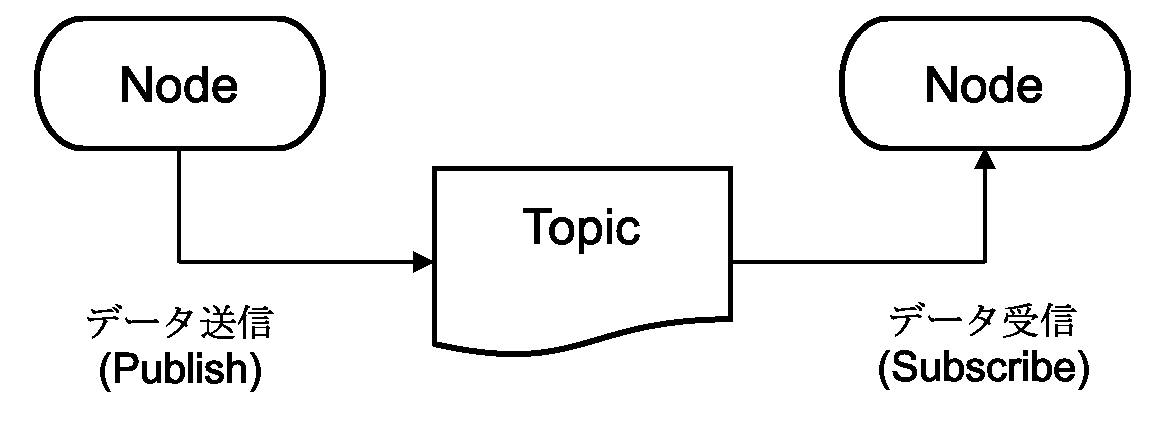
\includegraphics[width=0.5\hsize]{picture/eps/ros_topic.eps}
    \caption{ROSノードとトピックの概念}
    \label{fig::ros_topic}
\end{figure}



\begin{figure}[htb]
  \centering
    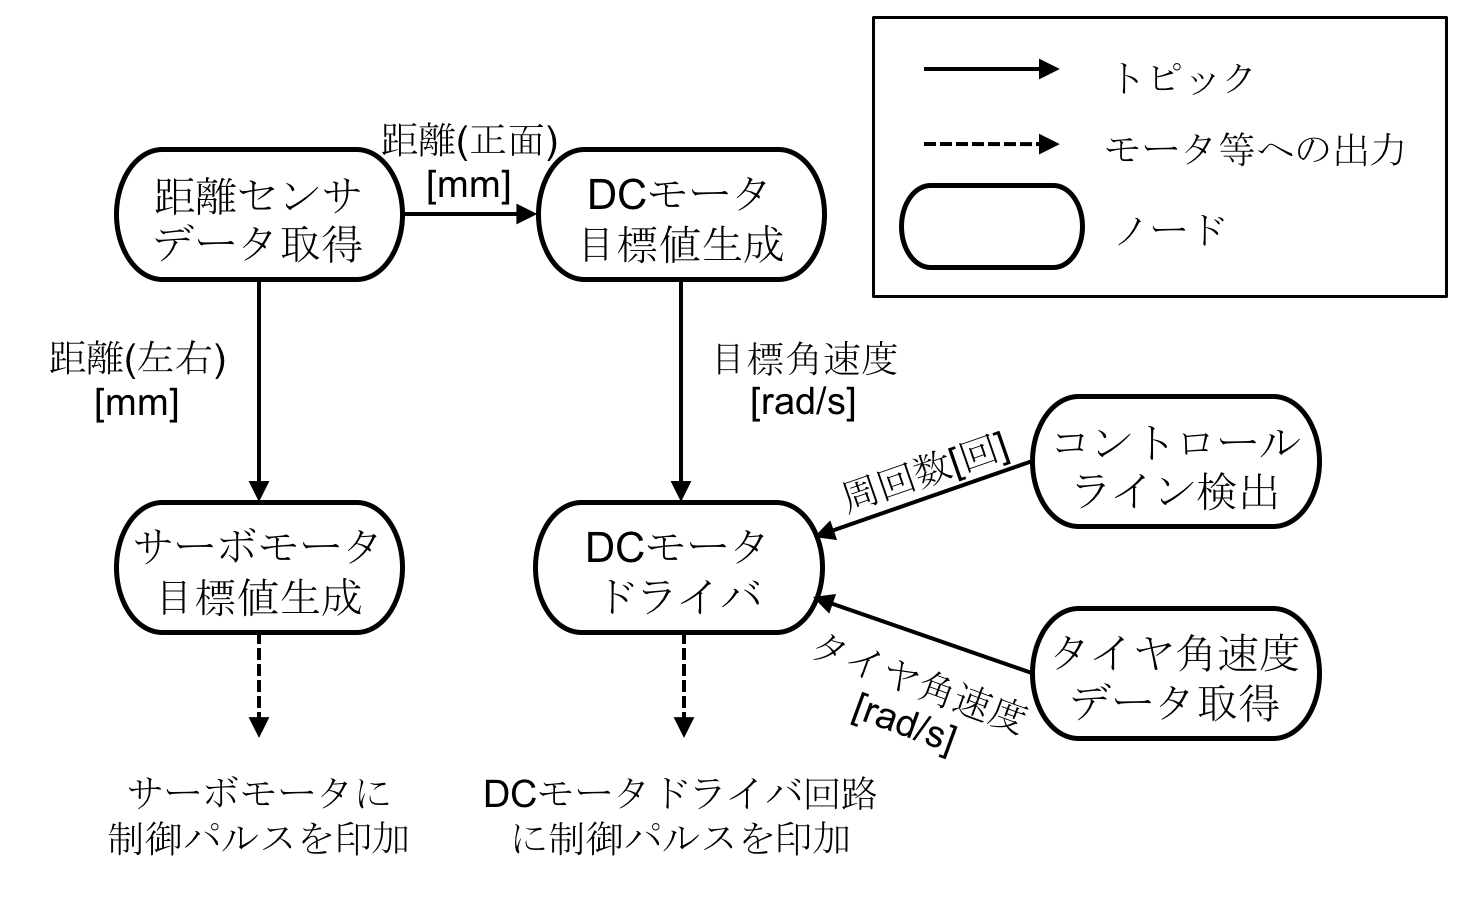
\includegraphics[width=0.8\hsize]{picture/eps/ros_nodes.eps}
    \caption{ROSノードとトピックの構成}
    \label{fig::ros_nodes}
\end{figure}

\newpage
\subsection{ROSノードとトピックの構成}
\refig{ros_nodes}に開発するROSノードとトピックの構成を示す.各ノードの役割は次の通りである.
\begin{description}

    \item[距離センサデータ取得] \mbox{} \\
      ロボカーの前方及び両側面に設置した距離センサからシリアルバス規格の一つである$\mathrm{I^2C}$を介して距離データを$\mathrm{[mm]}$単位で取得し外れ値処理や正規化を施した後にPublishする.
    \item[コントロールライン検出] \mbox{} \\
      ロボカーの後方下部に設置したフォトリフレクタによってコントロールラインを通過した回数をカウントしPublishする.

    \item[タイヤ角速度データ取得] \mbox{} \\
      ロボカーの後方に設置したロータリーエンコーダによって計測したタイヤの回転角を基に,タイヤの回転角速度を算出してPublishする.

    \item[DCモータ目標値生成] \mbox{} \\
      ロボカーの前方方向の距離データをSubscribeし,それをもとにDCモータに与える目標値を生成してPublishする.

    \item[ドライバ] \mbox{} \\
      DCモータに与える目標値,ロボカーの両側面の壁との距離,タイヤの角速度,周回数をSubscribeし,サーボモータの目標値を生成して,サーボモータを駆動させる.また,DCモータを目標値に追従するようなPI制御系によって駆動する.さらに,規定の周回数になるとロボカーを停止させる.


  \end{description}


\newpage
\subsection{DCモータのモデリング}
DCモータの代表的な等価回路を\refig{dcm_circit}に示す.\cite{dcmmodeling}ただし,モータへの入力電圧を$v\unit{V}$,電機子電流を$i_{a}\unit{A}$,電機子抵抗を$R_{a}\unit{\Omega}$,自己インダクタンスを$L_{a}\unit{H}$,誘起電圧定数を$K_{E}\unit{Vs/rad}$,電機子の回転角速度を$\omega_{m}\unit{rad/s}$,電機子に発生するトルクを$T\unit{Nm}$,負荷トルクを$T_L\unit{Nm}$,回転子と負荷の合成慣性モーメントを$J\unit{kg\cdot m^2}$とする.以下ではこの等価回路に沿ってDCモータの定式化を行う.

\refig{dcm_circit}より,DCモータの支配方程式は次のように書ける.
\begin{align}
v &= K_{E}\omega_{m} + R_{a}i_{a} + L_{a}\frac{di_{a}}{dt} \label{eq::dcm_v} \\
T &= J\frac{d\omega_{m}}{dt} + T_{L} \label{eq::dcm_t}
\end{align}

\refeq{dcm_v},\refeq{dcm_t}より\refig{dcm_block}のブロック線図を得る.
ここで,図中の$J$はモータ回転子の慣性モーメント$J_{M}$と負荷の慣性モーメント$J_{L}$の和を表し,
$K_{T}\unit{Nm/A}$はDCモータのトルク定数である.
\refig{dcm_block}より負荷を含まないDCモータ単体の伝達関数$G_{M}(s)$を求めると以下のようになる.
\begin{align}
G_{M}(s) &= \frac{\Omega_{m}(s)}{V(s)} = 
\frac{\cfrac{K_{T}}{(R_{a} + L_{a}s)J_{M}s}}{1 + \cfrac{K_{T}K_{E}}{(R_{a} + L_{a}s)J_{M}s}} \nonumber \\
 &= \frac{\cfrac{1}{K_{E}}}{1 + \cfrac{R_{a}J_{M}}{K_{T}K_{E}}s + \cfrac{L_{a}J_{M}}{K_{T}K_{E}}s^2} \label{eq::dcm_tf}
\end{align}

ただし,$\Omega_{m}(s) = \mathcal{L}\{\omega_{m}(t)\},V(s) = \mathcal{L}\{v(t)\}$である.

\refeq{dcm_tf}より,電流の増加を遅らせるインダクタンスと回転角速度の上昇を遅らせる慣性モーメントという2つのエネルギ蓄積素子が二次のダイナミクスをつくっている事がわかる.

\begin{figure}[htb]
  \centering
    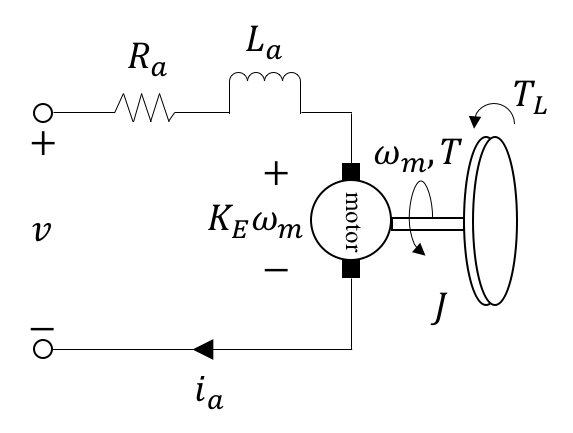
\includegraphics[width=0.5\hsize]{picture/eps/dcm_circit.eps}
    \caption{DCモータの等価回路}
    \label{fig::dcm_circit}
\end{figure}

\begin{figure}[htb]
  \centering
    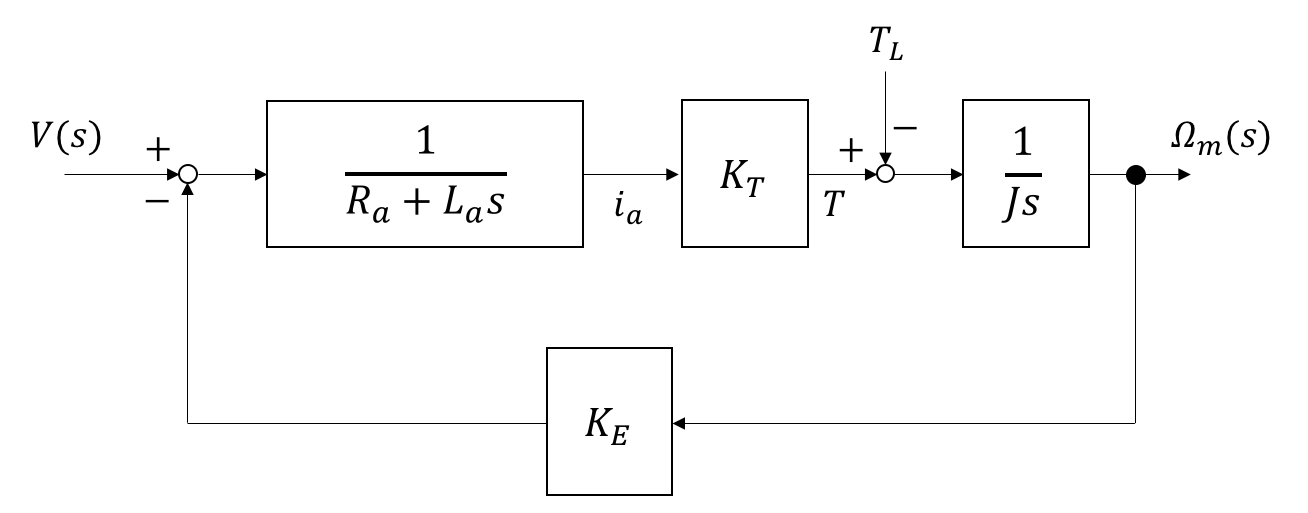
\includegraphics[width=1.0\hsize]{picture/eps/dcm_block_diagram.eps}
    \caption{DCモータのブロック線図}
    \label{fig::dcm_block}
\end{figure}

\newpage
\begin{figure}[h]
\centering
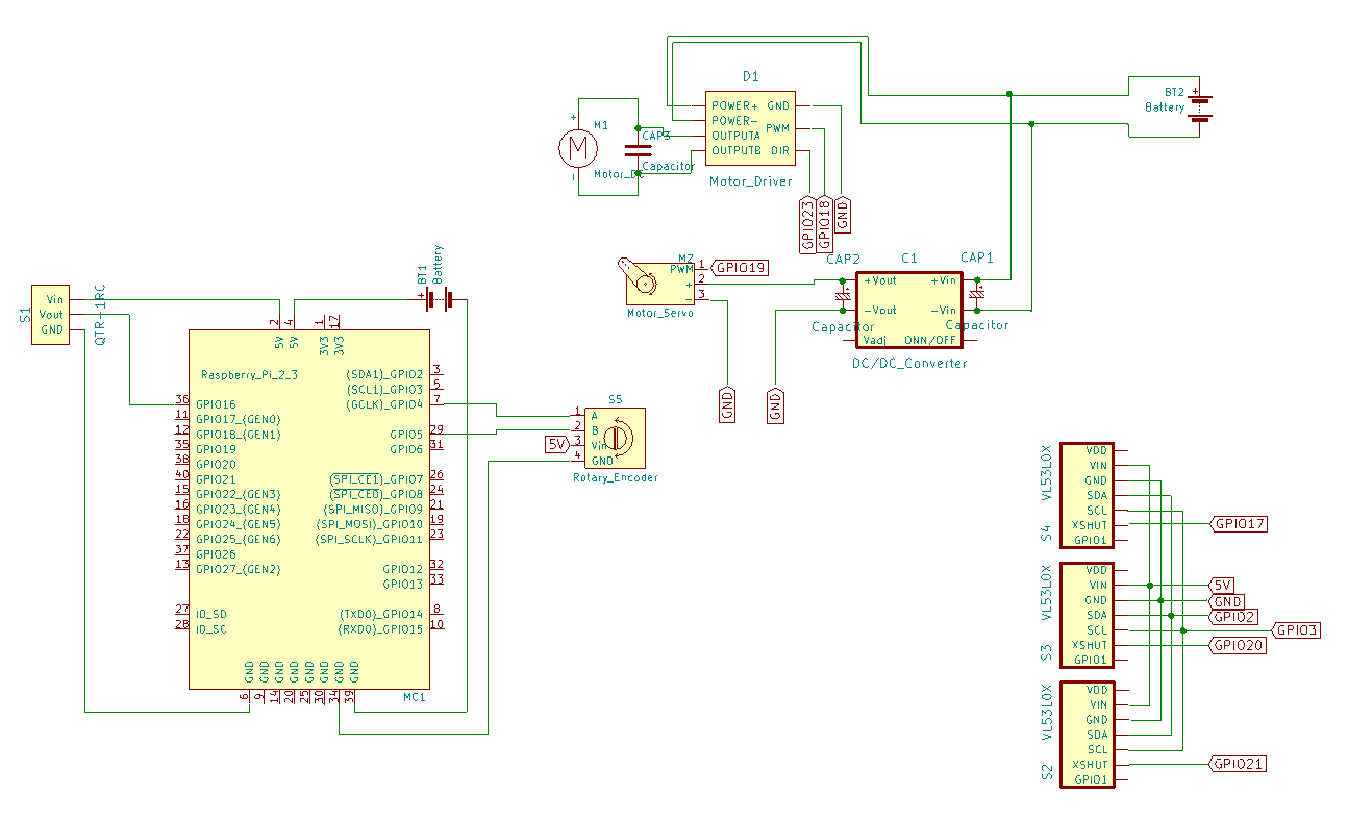
\includegraphics[scale=0.6]{picture/eps/ele_circuit_fig1.eps}
\caption{回路図}
\label{fig::overall_electric_circuit}
\end{figure}
\section{回路設計}
今回設計した回路を\refig{overall_electric_circuit},回路制作に使用した主要な部品の一覧を\reftab{circuit_parts}にそれぞれ示す.さらに各電子部品の仕様や構成について以下に示す.

\subsection{電源回路}
以下に示す仕様のようにRaspberryPi3 Model Bとサーボモータ,DCモータドライバではそれれぞれ定格電圧が異なるため同一の電源を用いることができない.そこで$7.2\unit{V}$バッテリと$5\unit{V}$バッテリの2つを用いている.
$7.2\unit{V}$バッテリはまず分流を行い,一方をDC-DCコンバータを用いて$7.2\unit{V}$から$5\unit{V}$に降圧してサーボモータに供給し,もう片方をDCモータドライバに供給している.$5\unit{V}$バッテリはRaspberryPi3 Model Bに電源を供給している.
\begin{description}
    \item[モータドライバ\textless MD10CR3\textgreater \cite{motordriver}]\mbox{}\\
    \vspace{-5mm}
        \begin{itemize}
            \item モータ電源電圧: DC $5\unit{V}-25\unit{V}$
            \item 最偉大電流  : $13\unit{A}$
            \item ロジック入力電圧: $3.3\unit{V}-5\unit{V}$
        \end{itemize}
    \item[サーボモータ\textless GWS03T/2BBMG\textgreater]\mbox{}\\
    \vspace{-5mm}
         \begin{itemize}
            \item 駆動電圧: DC $4.8\unit{V}-6\unit{V}$
        \end{itemize}
     \item[RaspberryPi3 ModelB\cite{rpi}]\mbox{}\\
     \vspace{-5mm}
         \begin{itemize}
            \item 電源: $5\unit{V}$,$2.5\unit{A}$
        \end{itemize}

\end{description}


\begin{table}
    \caption{電気回路用部品}
    \label{tab::circuit_parts}
    \begin{center}
    \footnotesize
   \begin{tabular}{ | l | l | c || l |}\hline
タイプ               &部品名                                         &数&用途   \\ \hline\hline
マイコン             &Raspberry Pi3 Model B                            &1&制御用           \\ \hline
DCモータ             &RP380-ST                                  &1&後輪モータ駆動用   \\    \hline
モータドライバ          &MD10C R3                                        &1&後輪モータ制御用   \\ \hline
距離センサ            &VL53L0X Time-of-Flight                           &3&距離計測用   \\ \hline
フォトリフレクタ         &QTR-1RC フォトリフレクタ・モジュール              &3&ゴールライン計測用   \\ \hline
DC-DCコンバータ          &BTD05-05S200D                                     &1&降圧用   \\ \hline
コンデンサ                &セラミックコンデンサ$1000\unit{pF}50\unit{V}$ &1&後輪モータのノイズ除去用   \\ \cline{2-4}
                          &OSコンデンサ $10\unit{V}47\unit{\mu F}$                          &2&DC-DCコンバータのノイズ除去用    \\ \hline
ロータリーエンコーダ   &RE30E-500-213-1                                   &1&ロボカーの速度計測用   \\ \hline
バッテリ             &Powers Max 4000 Ni-MH $7.2\unit{V}$                        &1&DCモータ,サーボモータ用の電源\\ \cline{2-4}
                          &$4000\unit{mAh}$ 6CELL ニッケル水素バッテリ                &1&Raspberry Pi3 ModelB用の電源    \\ \hline
サーボモータ           &GWS03T/2BBMG                                &1&ステアリング用   \\    \hline
 
	   \end{tabular} 
	\end{center}
\end{table}


\newpage

\begin{figure}[h!]
\centering
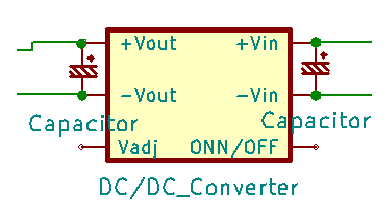
\includegraphics[scale=0.8]{picture/eps/ele_cap.eps}
\caption{DC-DCコンバータの回路図}
\label{fig::ele_cap}
\end{figure}

\subsection{DC-DCコンバータ}
本回路上で降圧を行うためにDC-DCコンバータを用いた.以下にその仕様を示す.DC-DCコンバータは内部でディジタルスイッチングを行っているため,ノイズが多い\cite{dcdc}.本回路ではこのようなノイズ成分を除去するために電解コンデンサ(OSコンデンサ$10\unit{V}47\unit{\mu F}$)を用いた\refig{ele_cap}の回路を作成した\cite{dcdcconverter}.
\begin{description}
    \item[DC-DCコンバータ\textless BTD05-05S200D\textgreater \cite{dcdcconverter}]\mbox{}\\
    \vspace{-5mm}
        \begin{itemize}
            \item 入力電圧: DC $4.5\unit{V}-9\unit{V}$
            \item 出力電圧: $0\unit{mA}-2000\unit{mA}$
            \item 出力電流: $3.3\unit{V}-5\unit{V}$
            \item 効率: 84 \%
        \end{itemize}
\end{description}




\newpage
\begin{thebibliography}{99}
 \bibitem{kurazume}
    表允晳,倉爪亮,渡邊裕太, "詳説 ROSロボットプログラミング-導入からSLAM・Gazebo・MoveItまで-", 
    Kurazume Laboratory, pp.15-18, (2015).

  \bibitem{ogura}
    小倉崇, "ROSではじめるロボットプログラミング", 工学社, pp.8-10, (2015).
  
  \bibitem{motor} 
  後閑哲也, "作る,できる/基礎入門 電子工作の素", 技術評論社, p181, (2009).
  
  \bibitem{motordriver} 
  Cytron technologies, "MD10C Enhanced 10Amp DC Motor Driver User's Manual Rev2.0 v1.0", 
  \textless https://www.robotshop.com/media/files/PDF/user-manual-md10c-v2.pdf\textgreater , 2018年6月2日アクセス.
  
  \bibitem{R380} 
  MABUCHI MOTOR, "Let's Motorize", 
  \textless https://www.mabuchi-motor.co.jp/motorize/branch/motor/\textgreater , 2018年6月3日アクセス.
  
  \bibitem{dcdcconverter} 
  SWITCH SCIENCE, "10Watt BTD Series", 
  \textless http://www.bellnix.co.jp/pdf/pdf/BTD.pdf\textgreater , 2018年6月2日アクセス.
  
  \bibitem{dcdc} 
  後閑哲也, "作る,できる/基礎入門 電子工作の素", 技術評論社, pp.84-85, p186, (2009).
  
  \bibitem{pololu}
   Pololu\quad Corporation,\quad "QTR-1RC\quad Reflectance\quad Sensor(2-Pack)",
   \textless https://www.pololu.com/product/2459 \textgreater , 2018年6月1日アクセス.
   
  \bibitem{tof_sensor1}
  SWITCH SCIENCE, "Pololu VL53L0X Time-of-Flight 距離センサモジュール"
  \textless https://www.switch-science.com/catalog/2869 \textgreater
  2018年6月1日アクセス.
  
  \bibitem{i2c}
  Philips\quad Semiconductors,\quad "$\mathrm{I^2C}$\hspace{0.5em}バス仕様書バージョン2.1"          
  \textless http://ekousaku.web.fc2.com/doc/I2C.pdf \textgreater
  \quad 2018年6月1日アクセス.
  
  \bibitem{dcmmodeling}
    坂本哲三, "電気機器の電気力学と制御", 森北出版, pp.164-168, (2007).
  

\end{thebibliography}

\end{document}
